\documentclass[conference]{IEEEtran}
\IEEEoverridecommandlockouts
\usepackage[utf8]{inputenc}
\usepackage[T1]{fontenc}
\usepackage{microtype}
\setlength{\emergencystretch}{1em}
\usepackage{amsmath,amssymb}
\usepackage{booktabs}
\usepackage{graphicx}
\usepackage{xcolor}
\usepackage{tikz}
\usepackage{cite}
\usepackage{xurl}
\usepackage[hidelinks]{hyperref}

\newcommand{\TEP}{TEP}
\newcommand{\PROTO}{\textsc{proto}}
\newcommand{\cond}[1]{\textsf{#1}}
\newcommand{\lu}{local-unseen}
\newcommand{\ls}{own-fault}

\begin{document}

\title{Benefits and Limits of Shared Knowledge\\
for LLM-Based Fault Diagnosis\\
under Extreme Label Skew}

\author{%
\IEEEauthorblockN{Luca Sorrentino\IEEEauthorrefmark{1},
Gabriele Piantadosi\IEEEauthorrefmark{2},
Antonio Galli\IEEEauthorrefmark{1},
Girolamo Di Francia\IEEEauthorrefmark{2} and
Carlo Sansone\IEEEauthorrefmark{1}}
\IEEEauthorblockA{\IEEEauthorrefmark{1}University of Naples Federico II,
Electrical Engineering and Information Technology Department, Napoli, 80125, Italy}
\IEEEauthorblockA{\IEEEauthorrefmark{2}ENEA CR-Portici,
Energy Technologies and Renewable Sources Department, Portici, 80055, Italy}
}

\maketitle

% ---------------------------------------------------------------------
\begin{abstract}
Industrial fault data may be unevenly distributed. We test an offline, non-iterative exchange inspired by Federation over Text (FoT) on the Tennessee Eastman Process: eight simulated clients each hold Normal data and one distinct fault class. Peers' faults are local-unseen to each receiver; its own class defines own-fault cases. A large language model (LLM) reads local examples and fixed, rule-based insights. A numerical nearest-class-mean (prototype) rule and fixed FedAvg reference use the same per-client development split. In a prespecified test on 256 new simulation runs, the LLM with peer insights had 64.7\% accuracy on local-unseen faults vs.\ 5.1\% with local examples alone; own-fault accuracy was 69.3\% vs.\ 85.4\%. Adding the receiver's own-class insight to the peer-insight prompt was associated with 20.8 percentage points (pp) higher own-fault accuracy (run-paired 95\% CI 14.9--26.8; $p<0.001$). In the same comparison, incorrect assignments to the receiver's fault on Normal cases were 99 vs.\ 69 of 512 decisions. Replacing peer insights with content-free text also showed a similar own-fault gain; this prompt contains no own-class insight, so it is not a direct control for the added own-class insight content. Against the prototype on local-unseen faults, the peer-insight LLM was 86.3~pp higher on fault 1 and 45.8~pp lower on fault 8 (both Holm-adjusted $p<0.001$). FedAvg reached 72.9\% pooled accuracy on local-unseen faults, above every LLM condition (at most 64.7\%). Text sharing thus showed gains over local examples, but its value varied by fault and receiver role and did not establish a general advantage over numerical references.

\end{abstract}

\begin{IEEEkeywords}
federated learning, label distribution skew, large language models, in-context learning, fault diagnosis, Tennessee Eastman Process, multivariate time series
\end{IEEEkeywords}

% ---------------------------------------------------------------------
\section{Introduction}
\label{sec:intro}
Industrial sites may hold examples of their own faults but none of the faults observed at other sites; we model each site as a client. In the extreme label-skew pattern we study here, each client has Normal data and one distinct fault class. Federated learning can combine model updates without pooling raw client records~\cite{mcmahan2017fedavg}, but severe label skew complicates training~\cite{li2022noniid} and parameter updates also do not directly expose the diagnostic observations behind them. Sharing concise textual observations makes them inspectable, though not private by itself. We study this setting on the Tennessee Eastman Process (\TEP{})~\cite{downs1993tep,bathelt2015tep},a simulated chemical-process benchmark.

Federation over Text (FoT)\cite{yao2026fot} takes this route: iteratively distills clients' language-model reasoning traces into a shared insight library~\cite{yao2026fot}. Our offline exchange is simpler and neither implements FoT nor runs an online federation protocol: a fixed rule renders one textual insight from recurring observations in each client's separate development data, and a large language model (LLM) reads those insights once as context. We compare it with a numerical nearest-class-mean rule, which assigns a case to the closest mean of fixed features (a prototype), and a fixed FedAvg reference. Learned prototypes have been studied for federated fault diagnosis under label skew~\cite{fan2025prototype}; federated zero-shot diagnosis has also shared semantic fault descriptions~\cite{li2023fedzsl}. Neither study directly compares rule-based insights read in context by an LLM with simple numerical class means and FedAvg on the same cases. We therefore ask how peer insights relate to diagnosis of local-unseen faults, how an own-class insight relates to recognition of the receiver's fault, and how those outcomes compare with numerical references.

Eight simulated \TEP{} clients each hold Normal data and one distinct fault. For a receiver, another client's fault is \emph{local-unseen}; its own fault and Normal operation are separate outcomes. Each five-hour simulation case is presented to all eight receivers, but the simulation run is the unit of inference. Motivated by an exploratory cohort of 96 runs, two prespecified test families on 256 new runs examine (i) the own-fault difference when the LLM receives an own-class insight in addition to peer insights, and (ii) its difference from the prototype rule on fault 1 and fault 8, with Holm correction. Those fault classes were selected from the exploratory cohort; all eight remain in pooled summaries. Other conditions, Normal decisions, abstentions and malformed responses are reported descriptively. A supplementary LLM supplies an exploratory comparison on the same cases: it received the same messages and output schema, while other generation and serving controls differed.

With peer insights, accuracy on local-unseen faults was 64.7\% vs.\ 5.1\% with local examples alone, while own-fault accuracy was lower (69.3\% vs.\ 85.4\%). Adding an own-class insight to the peer prompt was associated with 20.8~pp higher own-fault accuracy, alongside more Normal cases incorrectly assigned the receiver's fault label (99 vs.\ 69 of 512 decisions). Compared with the prototype, the peer-insight LLM was 86.3~pp higher on fault 1 and 45.8~pp lower on fault 8; fixed FedAvg reached 72.9\% pooled local-unseen accuracy, above every LLM condition. Our contribution is a prespecified, run-paired evaluation of in-context
collaboration for LLM-based fault diagnosis under extreme label skew.
Here, collaboration means that a receiver reads other clients' insights (peer insights) in its prompt; some conditions also add an insight from the receiver's own class.
We assess own-fault and local-unseen accuracy, Normal false alarms and
abstentions, and performance relative to numerical references, reporting
adverse results alongside favorable ones.
Because the systems receive unequal information, their performance gaps
do not isolate the effect of textual content.
The results concern simulated classification, not privacy or industrial
deployment.

\section{Related Work}
\label{sec:related}

\paragraph{Parametric and prototype-based federation}
\mbox{FedAvg}~\cite{mcmahan2017fedavg} averages model parameters across clients. Li et al.~\cite{li2022noniid} find label skew the most challenging of the non-identically distributed (non-IID) settings they study; their quantity-based label imbalance restricts the number of labels per client. Our class-disjoint faults with shared Normal instantiate that form of label skew, with two labels per client rather than their hardest one-label setting. FedProto~\cite{tan2022fedproto} forms class prototypes as means of learned embeddings; a server combines them to guide subsequent local training, and Tan et al. also describe nearest-prototype inference. In mechanical fault diagnosis, Fan et al.~\cite{fan2025prototype} study clients with a common Normal class and disjoint fault classes, using learned global prototypes to recognize local-unseen classes. Li and Zhao~\cite{li2023fedzsl} share a semantic knowledge base derived from human fault descriptions among clients with disjoint faults, train data--attribute models and aggregate their diagnostic knowledge. They distinguish locally and globally unseen faults and report seen/unseen accuracy with and without aggregation; their evaluated label sets contain faults only, without Normal or abstention. Our prototype rule classifies by mean absolute (L1) distance to class means of fixed features, without representation learning or iterative optimization: a simple distributable rule, not a state-of-the-art federated baseline. We also evaluate FedAvg on the same clients and test cases: post hoc on the exploratory cohort and as one fixed reference in the present test (Section~\ref{sec:conditions}).

\paragraph{Textual federation and in-context collaboration}
FoT~\cite{yao2026fot} is the reference method: in each round, clients send reasoning traces to a server, which distills them into an insight library used by agents in context. Related approaches exchange natural-language compendia~\cite{wu2024fical}, iteratively refine answers~\cite{wang2025fedicl}, aggregate prompts optimized locally with textual gradients~\cite{chen2025fedtextgrad}, or study social learning between language models~\cite{mohtashami2023social}. Fed-S2~\cite{zhang2026feds2} uses a frozen LLM with retrieval from client-uploaded embedding prototypes and descriptions for bearing diagnosis; its reported zero-shot test preloads prototypes for classes excluded from training. Our peer insights are rendered once by a fixed rule-based procedure from recurring observations in each contributing client's development data. No LLM writes them, and in the peer-insight conditions there is no cross-client distillation, server-side merging or later revision. One condition, \cond{AGG}, adds a single server-side step in which the LLM synthesizes the eight insights into one library (Section~\ref{sec:conditions}). Server-side aggregation of client text is not new: FICAL concatenates client compendia~\cite{wu2024fical}, and FedTextGrad concatenates or summarizes client prompts over rounds~\cite{chen2025fedtextgrad}. \cond{AGG} is a single-cycle control inspired by FoT's server-side distillation, not FoT.

\paragraph{Trade-offs of shared knowledge}
In parametric federation, personalized and generic accuracy compete: improving one can degrade the other.~\cite{chen2022fedrod}. For LLMs, retrieved context can lower accuracy, even on questions answered correctly without it~\cite{mallen2023trust,yoran2024robust}. These precedents suggest that shared knowledge should not be judged on one outcome alone; we report the prespecified own-fault and Normal outcomes alongside local-unseen accuracy. Longer inputs can also affect LLM reasoning on otherwise identical tasks~\cite{levy2024same}, so we report prompt-token use (Section~\ref{sec:cost}) and treat length as a confound we cannot remove (Section~\ref{sec:limits}).

\paragraph{Time series, language and \TEP{} diagnosis}
Work linking time series and language includes structured program representations~\cite{kim2026t2sp} and signals-to-semantics zero-shot fault diagnosis (S2S-FDD)~\cite{li2025s2sfdd}. The \TEP{} simulator is a standard process-monitoring benchmark~\cite{downs1993tep,bathelt2015tep}. On \TEP{}, FaultExplainer~\cite{khan2025faultexplainer} gives an LLM principal component analysis (PCA)-based detection output and the top contributing variables; its unseen-fault scenario withholds a list of known root causes from the prompt, whereas \lu{} here means the receiving client has no local examples of the fault. S2S-FDD and FaultExplainer are centralized: no knowledge passes between clients. In simulated fault diagnosis, Lee et al.~\cite{lee2025agentic} report stronger LLM anomaly detection with summarized statistical inputs than with raw sensor readings, at best approaching a rule-based statistical baseline in $F_1$ score. Kim~\cite{kim2026complementarity} supplies a trained classifier's label to LLMs on \TEP{} cases and finds the combined output below the classifier alone. That centralized integration passes a specialist prediction rather than peer insights. Our rule-based procedure is deterministic and frozen; we make no claim about learned text representations.

We test own-class and peer insights as separate prompt components and assess their joint gains and costs across own-fault, local-unseen and Normal cases. Comparisons with the prototype rule and FedAvg show how the text-based conditions perform beyond the local-example baseline; neither FoT nor FedProto is evaluated as a complete algorithm.

% ---------------------------------------------------------------------
\section{Simulated Setting and Compared Systems}
\label{sec:method}

Figure~\ref{fig:method-flow} shows the text and numerical paths, including both the prototype and FedAvg references. The following subsections define the offline construction and decision-time inputs.

% Method overview (TikZ, one column, basic TikZ only). Both panels read top to bottom.
% Arrows = derivation and use of stored artifacts, not communication; dashed = peer insights (some conditions only).


\begin{figure}[t]
\centering
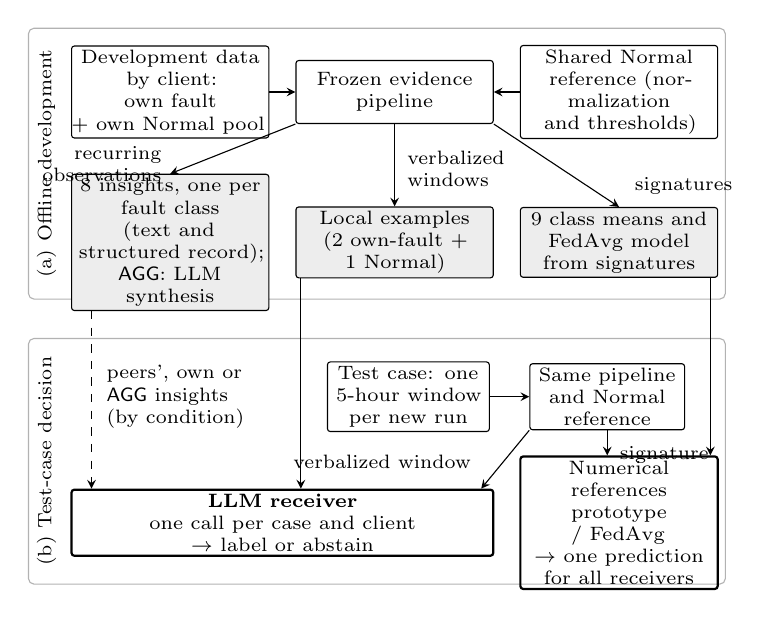
\begin{tikzpicture}[x=1mm,y=1mm,>=stealth,
  box/.style={draw,rounded corners=1pt,align=center,font=\scriptsize,inner sep=1.5pt,text width=24mm,minimum height=8mm},
  art/.style={box,fill=gray!14},
  sys/.style={box,thick},
  lab/.style={font=\scriptsize,inner sep=1pt,align=left}]
% panel frames and side titles
\draw[gray!60,rounded corners=2pt] (0,-24.8) rectangle (88.5,9.6);
\draw[gray!60,rounded corners=2pt] (0,-61) rectangle (88.5,-29.8);
\node[font=\scriptsize,rotate=90] at (2.3,-7.6) {(a) Offline development};
\node[font=\scriptsize,rotate=90] at (2.3,-45.4) {(b) Test-case decision};
% (a) data and pipeline
\node[box] (cli) at (18,1.5) {Development data\\by client: own fault\\+ own Normal pool};
\node[box] (pipe) at (46.5,1.5) {Frozen evidence\\pipeline};
\node[box] (ref) at (75,1.5) {Shared Normal\\reference (normalization\\and thresholds)};
\draw[->] (cli) -- (pipe);
\draw[->] (ref) -- (pipe);
% (a) stored artifacts
\node[art] (ins) at (18,-17.6) {8 insights, one per\\fault class (text and\\structured record);\\\cond{AGG}: LLM synthesis};
\node[art] (loc) at (46.5,-17.6) {Local examples\\(2 own-fault +\\1 Normal)};
\node[art] (mean) at (75,-17.6) {9 class means and\\FedAvg model\\from signatures};
\draw[->] (pipe.south west) -- (ins.north);
\draw[->] (pipe.south) -- (loc.north);
\draw[->] (pipe.south east) -- (mean.north);
\node[lab,anchor=east,align=right] at (17.3,-7.6) {recurring\\observations};
\node[lab,anchor=west] at (47.7,-8.2) {verbalized\\windows};
\node[lab,anchor=west] at (76.6,-10.4) {signatures};
% (b) test case and pipeline
\node[box,text width=19.5mm] (win) at (48.25,-37.2) {Test case: one\\5-hour window\\per new run};
\node[box,text width=18.6mm] (pipe2) at (73.5,-37.2) {Same pipeline\\and Normal\\reference};
\draw[->] (win) -- (pipe2);
% (b) the two systems
\node[sys,text width=52.5mm] (llm) at (32.25,-53.2)
  {\textbf{LLM receiver}\\one call per case and client\\$\rightarrow$ label or abstain};
\node[sys] (proto) at (75,-53.2)
  {Numerical references\\prototype / FedAvg\\$\rightarrow$ one prediction\\for all receivers};
% stored artifacts used at decision time
\draw[->,dashed] (8,0 |- ins.south) -- (8,0 |- llm.north);
\draw[->] (34.6,0 |- loc.south) -- (34.6,0 |- llm.north);
\draw[->] (86.6,0 |- mean.south) -- (86.6,0 |- proto.north);
\node[lab,anchor=west] at (9.5,-37.2) {peers', own or\\\cond{AGG} insights\\(by condition)};


% test case to the two systems
\draw[->] (pipe2.south west) -- (57.5,0 |- llm.north);
\node[lab,anchor=east] at (56.6,-45.4) {verbalized window};
\draw[->] (pipe2.south) -- (pipe2.south |- proto.north);
\node[lab,anchor=west] at (74.7,-44.6) {signature};
\end{tikzpicture}
\caption{Offline development and test-case decision paths. Arrows denote derivation and use of stored artifacts, not communication between clients.}
\label{fig:method-flow}
\end{figure}

\subsection{Clients, labels and units of analysis}
Eight simulated clients observe the same \TEP{} plant, each owning one fault class: three step changes (F1--F3), two random variations (F8, F10), one slow drift (F13) and two sticking valves (F14, F15)~\cite{downs1993tep}. The development pool is the labeled data from earlier simulation runs that all systems use to build their knowledge (insights, class means and FedAvg parameters); test cases come from separate runs. It is partitioned by client: each client has labeled development data for its own fault and its own Normal pool of 40 windows from five runs. The shared Normal reference consists of separate development Normal data, distinct from the clients' Normal pools; it is not private client training data, but its use departs from strict federation (Section~\ref{sec:limits}). The label space is $\{F1,F2,F3,F8,F10,F13,F14,F15,\text{Normal}\}$; a system outputs one label or abstains.

A \emph{case} is a 5-hour window from one run. Each case is paired with all eight clients, the receivers in the LLM conditions. A fault case yields one \emph{own-fault} pair with the client that owns its true fault class and seven \emph{\lu} pairs with the other clients; a Normal case yields eight \emph{Normal} pairs. The insight conditions simulate access to stored insights; no communication protocol is executed for them.

\subsection{Shared evidence pipeline}
The LLM and numerical references use one frozen evidence pipeline. Each 5-hour window has 300 one-minute samples for each of 41 measured variables (XMEAS). For each variable, the pipeline computes four statistics: mean shift (``level shift'' in the generated text), slope (linear trend), residual variability (standard deviation after linear detrending) and sample-to-sample variation (standard deviation of successive differences). It normalizes these statistics using the shared Normal reference and compares each with a fixed threshold calibrated on the same reference. Rapid variability is flagged only when both the residual and sample-to-sample statistics exceed their thresholds; an overall dispersion ratio is computed separately.

For the LLM, the pipeline renders each sensor window from a simulated run as a \emph{verbalized window}, a rule-generated English textual description of the window. It names the leading variable (the largest above-threshold magnitude) for each statistic (or says none), adds the leading variable for rapid variability when present and reports the largest dispersion ratio (window standard deviation divided by reference standard deviation). From the same evidence, the pipeline builds a 697-component numerical signature (feature vector) for both numerical references, with 17 fields per variable: four each for mean shift and slope (active fraction, sign balance, late-active fraction and longest same-sign run) and three each for residual variability, sample-to-sample variation and rapid variability (active fraction, late-active fraction and longest run). For a single window, these fields record which thresholds fired and their signs, not magnitudes. The signature spans all variables but excludes the dispersion ratio, so the two representations of the case differ.

The test case's verbalized window includes the absolute observed interval (hours) as fixed-onset context (faults begin at hour 25), but no fault label, run or stream ID, or file name. The interval does not identify the fault; local examples and any peer insights are labeled.

\subsection{Class insights from recurring observations}
For each fault class, 40 development windows from five runs are scanned over three time spans (25--65, 25--35 and 35--65~h) for candidate observations. Candidates name the most frequent leading variable for mean shift, slope, residual variability, sample-to-sample variation or overall dispersion, or note no threshold exceedances. A candidate is retained as a recurring observation if it holds in at least half the windows of its span. A shorter-span candidate is nevertheless discarded when it repeats the variable, or the all-quiet observation, of a retained full-span candidate of the same kind; 30 of 144 were retained. Each retained observation also reports its frequency in the contributing client's Normal development windows for that span. F3 and F15 produced only an all-quiet observation, which also describes most Normal windows.

A fixed rule-based procedure renders the retained observations as one insight per fault class in two forms: natural-language text and a structured record. Each insight comes from its class owner's development pool and can serve as that receiver's own-class insight or as a peer insight for another receiver. Both forms keep a class-bearing ID and name the class. A parse-back check confirms that both renderings contain the same 30 observations and headers, but does not show that an LLM uses them in the same way.

An excerpt from the actual \texttt{P05-INS-F1} insight, in natural language: ``Between 25 and 65 h, the largest above-threshold level shift is on XMEAS-1 in 40 of 40 development windows of F1 (positive in 40, negative in 0).'' The structured record includes \texttt{"observation": "largest above-threshold level shift"}, \texttt{"variable": "XMEAS-1"}, \texttt{"class\_windows": 40}, \texttt{"positive": 40} and \texttt{"negative": 0}. Both full renderings also note that this occurs in 0 of 40 Normal development windows of the contributing client; other F1 observations and fields are omitted.

\subsection{Conditions and numerical references}
\label{sec:conditions}
All seven conditions for the primary LLM use the same open-weight model (\texttt{qwen3.5-122b}, serving Qwen3.5-122B-A10B-FP8~\cite{qwen2026model}, hereafter the LLM) on a local inference service, with a common system-prompt template, the receiver's local block, the test case's verbalized window and strict four-field JSON output (\texttt{predicted\_label}, \texttt{abstain}, \texttt{used\_insight\_ids}, \texttt{reasoning\_summary}). Each receiver's fixed local block holds three local examples (in-context demonstrations): two verbalized windows of its own fault and one from its own Normal pool, at window positions fixed before any content was inspected. Generation uses temperature 0 and seed 20260927, with a 1,024-token thinking budget and up to 2,048 completion tokens. The fixed pre-test parser rejects \texttt{reasoning\_summary} strings longer than 1,200 characters, although this cap is absent from the transmitted JSON schema; Section~\ref{sec:results} examines its removal. The system prompt differs only in its ID instruction: \cond{AGG} requests common-library entry IDs; the other conditions request peer insight IDs. Conditions vary in the insight block after the local examples. When present, the own-class insight precedes any peer insights, which appear in fixed fault-number order:
\begin{itemize}[\IEEEsetlabelwidth{\cond{FULL}}]
\item[\cond{A0}] no insights (local-only);
\item[\cond{B0}] seven peers' natural-language insights;
\item[\cond{FULL}] \cond{B0} plus the receiver's own-class insight in natural language, so that the receiver reads all eight insights;
\item[\cond{SELF}] \cond{A0} plus the same own-class insight;
\item[\cond{AGG}] in place of the insights, one library that the LLM synthesized from the eight insights;
\item[\cond{S0}] structured records encoding the same seven peer insights as \cond{B0};
\item[\cond{PL0}] \cond{B0} with its seven peer insights replaced by generic process-monitoring text of the same byte length, but not the same token count (placebo).
\end{itemize}
\cond{S0} and \cond{PL0} ran in a later pass than \cond{B0}. \cond{S0} also produces longer prompts, so its comparison with \cond{B0} does not isolate format. \cond{A0}, \cond{B0}, \cond{SELF} and \cond{FULL} cross peer-insight presence with own-class insight presence ($2\times2$).

The \cond{AGG} library was written once, before any test use, from the eight natural-language insights alone: in two requests the LLM listed relations between insights and wrote 13 entries, eight on single classes and five contrasting two classes. After one permitted correction cycle it was accepted on a source audit, not on diagnostic accuracy. Both LLMs used this same stored library.

The prototype rule, denoted \PROTO{}, is a non-LLM rule fixed on development data, using class means computed from development signatures: 40 windows for each of eight faults and 320 pooled Normal windows. For each case, \PROTO{} selects the class with minimum mean absolute distance over 697 components, abstaining if another class is within $10^{-12}$ of the minimum. It outputs one receiver-independent prediction per case, copied across receiver pairs for paired evaluation.

The new test includes FedAvg as a second numerical reference: logistic regression on the 697-component signatures, trained on the eight clients' development data (50 rounds, five local epochs per round, learning rate 0.3, no regularization, five seeds, class probabilities averaged). Its settings were chosen by cross-validation on development data, but this recipe was named as the reference only after its exploratory-cohort results were known. Like \PROTO{}, it predicts once per case; unlike \PROTO{}, it always issues a class label and cannot abstain. The parameters used are not those behind the exploratory-cohort results: they were rebuilt from development data alone and frozen before any new test case was scored (Section~\ref{sec:limits}).

The systems share test cases but differ in decision-time information. \PROTO{} uses all nine class means, including the receiver's own fault mean and the mean of 320 pooled Normal windows; FedAvg is trained on all eight clients' development pools. An LLM receiver sees one local Normal example and, in insight conditions, Normal frequencies attached to the supplied fault facts, but no separate Normal insight. These differences matter when interpreting false alarms. We compare complete systems with unequal decision-time information.

The supplementary LLM, \texttt{gpt-oss-120b}~\cite{gptoss2025model}, receives the same system/user messages, output schema, temperature and seed on every matched case, receiver and condition. Its other generation and serving settings are: top-$p$ 1, unrestricted top-$k$, low reasoning effort, a 4,096-token output cap, a 16,384-token context and four concurrent requests. Both inference services report vLLM 0.27.1~\cite{kwon2023vllm}. Cross-model comparisons therefore describe configured systems rather than isolate model-weight effects (Section~\ref{sec:limits}).

\subsection{Reused development components}
\label{sec:provenance}
Reused components have pinned source hashes: the qualified Simulink model with independent random streams for fault injection; frozen features, thresholds and verbalization (current English wording); labels and fault ownership; the 80-run development pool; and the shared Normal reference. PROTO matches its source rule and development outputs. Earlier evaluation runs, predictions and results are not pooled into either cohort; from the exploratory cohort, the new evaluation takes only the hypotheses, conditions and FedAvg reference (Section IV).(Section~\ref{sec:protocol}).

% ---------------------------------------------------------------------
\section{Evaluation Design}
\label{sec:protocol}
The benchmark has two primary test families:
\cond{FULL}$-$\cond{B0} on own-fault accuracy (Family~A), and
\cond{B0}$-$\PROTO{} on local-unseen F1 and F8, with Holm correction
(Family~B).
Descriptive comparisons assess peer-insight access, the own-class
insight without peers, and their interaction.
Additional controls examine content-free replacement of peer insights
(\cond{PL0}), structured rendering (\cond{S0}), and single-cycle
synthesis (\cond{AGG}).
These controls do not isolate the semantic contribution of the added
own-class insight.
Normal false alarms, false own-label assignments, abstentions and
invalid responses describe diagnostic costs alongside accuracy;
comparisons with numerical references assess competitiveness.

\subsection{Cohorts and window selection}
The 80-run development pool, shared Normal reference, and post-onset 5-hour window rule were fixed before either evaluation cohort. The 96-run exploratory cohort (eight per fault, 32 Normal) supplied three prespecified local-unseen contrasts, analyzed before planning the new evaluation and presented only as context. The new cohort contains 256 disjoint-stream runs (24 per fault, 64 Normal), a size informed by conditional exploratory-cohort planning scenarios without a power guarantee. Runs last 65 hours; faults begin at hour 25, and eight half-open 5-hour windows cover $[25,65)$~h. For within-class run position $k$ and class offset $o_\ell$, the selected ordinal is $j=1+((k-1+o_\ell)\bmod 8)$, giving interval $[25+5(j-1),30+5(j-1))$. Offsets are 0--7 in the listed fault order and 0 for Normal. Each fault covers every window three times and Normal eight times; all 256 runs passed technical checks without replacement.

This produces 192 own-fault, 1,344 local-unseen and 512 Normal receiver pairs per condition. The seven LLM conditions (\cond{A0}, \cond{B0}, \cond{FULL}, \cond{SELF}, \cond{AGG}, \cond{S0}, \cond{PL0}) received 14,336 requests in total. For each case--receiver pair, the first pass interleaved \cond{A0}, \cond{B0}, \cond{FULL}, \cond{SELF} and \cond{AGG} in that order; a subsequent pass interleaved \cond{S0} and \cond{PL0}. Both passes preceded evaluator-truth opening. The supplementary LLM ran the same seven conditions on this grid, with different generation and serving controls.

\subsection{Outcomes and run-level inference}
Exact-label correctness at the fixed planned denominator is primary: no top-$k$ or alias credit, voting, or content-based retries. Each planned case--receiver--condition combination contributes one response; abstentions, parser rejections, truncations and missing responses count as non-correct and are reported separately. Wrong-fault labels, faults missed as Normal, and false alarms on Normal remain distinct from non-answers. A false own-label assignment predicts the receiver's fault when the true class differs. HTTP 200 alone is not a correct diagnosis. Let $Y_{a,r,c}$ be one for a valid exact-label answer by condition $a$ on run $r$ and receiver $c$, and zero otherwise. For a contrast $a-b$ and receiver set $C_r$,
\begin{equation}
d_r=\frac{1}{|C_r|}\sum_{c\in C_r}(Y_{a,r,c}-Y_{b,r,c}),\qquad
\widehat\Delta=\frac{1}{K}\sum_{f=1}^{K}\bar d_f.
\end{equation}
The set $C_r$ contains one owner, seven non-owners or eight receivers for own-fault, local-unseen or Normal. Fault contrasts weight included classes equally after averaging runs within class; Normal averages its 64 run differences. The physical run is the inferential unit.

For Family~A, $K=8$, $n_f=24$, and
\begin{equation}
\widehat{\mathrm{SE}}^2=\frac{1}{K^2}\sum_f v_f,\quad
v_f=\frac{s_f^2}{n_f},\quad
\nu=\frac{(\sum_f v_f)^2}{\sum_f v_f^2/(n_f-1)},
\end{equation}
where $s_f^2$ is the sample variance of the run differences. Family~A tests \cond{FULL}$-$\cond{B0} on 192 own-fault runs with a class-stratified two-sided $t$ test and 95\% $t$ interval using Welch--Satterthwaite degrees of freedom~\cite{welch1947,satterthwaite1946}.

Family~B tests \cond{B0}$-$\PROTO{} separately on F1 and F8 local-unseen runs, each averaged over seven receivers. Each fault's 24 run differences permit an exact whole-run sign-flip test over all $2^{24}$ assignments, including ties in the two-sided tail~\cite{winkler2014permutation}. Exactness requires run-wise sign invariance. Holm adjusts the two Family~B tests~\cite{holm1979}. Each family has its own two-sided $\alpha=0.05$; no joint 0.05 claim is made.

The three prespecified descriptive partitions are all eight faults, the six excluding F1/F8, and F1/F8 alone. Other condition comparisons are descriptive too; selected contrasts also use the class-stratified $t$ interval above, explicitly marked $t$ in the results. Pointwise percentile intervals use 20,000 within-fault run resamples, carrying all conditions and receivers together; Normal resamples its whole runs. These are run-level, not receiver-level, resamples~\cite{field2007bootstrap}.

The planned descriptive contrasts are \cond{B0}$-$\cond{A0}, \cond{SELF}$-$\cond{A0}, \cond{FULL}$-$\cond{SELF}, their $2\times2$ interaction, \cond{AGG}$-$\cond{FULL}, \cond{S0}$-$\cond{B0}, \cond{PL0}$-$\cond{B0}, and \cond{B0} against both numerical references. Two outcome-blind, point-only sensitivities were fixed before truth opening: dropping the whole run whose target text matches the F2 receiver's labeled example, and the lexicographically larger case ID from each of four duplicate target-text pairs, again as whole runs. Each exclusion applies across conditions and receivers; neither changes fixed-denominator results or adds tests or intervals. No equivalence margin was set. The dated local primary specification preceded new run generation; exploratory results motivated its hypotheses. The gpt-oss analysis was fixed after LLM requests began and remains exploratory descriptive. No case was replaced based on diagnostic outcomes.


\section{Results}
\label{sec:results}
All 14,336 primary-LLM requests returned HTTP 200 on the first attempt: 11,912 valid labeled answers, 2,343 abstentions, 43 parser rejections and 38 truncations. All remain in the fixed denominators (Tables~\ref{tab:t2main}--\ref{tab:t2arms}). Families A/B precede controls and the supplementary LLM. Other contrasts are descriptive: partition intervals use percentile bootstrap, intervals marked $t$ use stratified-$t$ summaries, and Normal contrasts are point estimates. These 95\% intervals are pointwise and unadjusted, with no additional tests.

With peer insights, local-unseen accuracy was 869/1,344 (64.7\%) in \cond{B0}, vs.\ 69/1,344 (5.1\%) in local-only \cond{A0}: $+59.5$~pp (95\% $t$ interval $[+56.7, +62.3]$). Own-fault accuracy was lower, 133/192 vs.\ 164/192 ($-16.1$~pp; $[-22.0, -10.2]$).

\begin{table*}[!t]
\centering\footnotesize
\caption{Prospectively specified 256-run test. Accuracy is in percent and contrasts in percentage points (pp) at the fixed denominator. Family A uses 192 own-fault physical runs; Family B uses 24 runs per fault, averaging seven local-unseen receivers within run. The gpt-oss rows are exploratory descriptive, not additional tests.}
\label{tab:t2main}
\setlength{\tabcolsep}{4pt}
\begin{tabular}{llrrl}
\toprule
Configured system / contrast & Outcome & Difference (pp) & Accuracies (\%) & Interval or test \\
\midrule
Qwen \cond{FULL}$-$\cond{B0} & Own-fault & $+20.8$ & 90.1 / 69.3 & 95\% CI $[+14.9,+26.8]$; $p=4.65\times10^{-10}$ \\
Qwen \cond{B0}$-$\PROTO{}, F1 & Local-unseen & $+86.3$ & 98.8 / 12.5 & Holm $p=1.91\times10^{-6}$ \\
Qwen \cond{B0}$-$\PROTO{}, F8 & Local-unseen & $-45.8$ & 37.5 / 83.3 & Holm $p=9.45\times10^{-4}$ \\
Qwen \cond{B0}$-$\PROTO{}, all faults & Local-unseen & $+3.7$ & 64.7 / 60.9 & Descriptive pointwise 95\% $[+0.1,+7.4]$ \\
gpt-oss \cond{FULL}$-$\cond{B0} & Own-fault & $+22.9$ & 62.0 / 39.1 & Descriptive pointwise 95\% $[+16.7,+29.2]$ \\
gpt-oss \cond{B0}$-$\PROTO{} & Local-unseen & $-9.5$ & 51.4 / 60.9 & Descriptive pointwise 95\% $[-13.6,-5.4]$ \\
\bottomrule
\end{tabular}

\end{table*}

\begin{table*}[!t]
\centering\footnotesize
\caption{LLM operational accuracy by receiver role and response state, all at planned denominators (2,048 pairs per LLM condition). Abstentions, parser rejections and truncations are retained as non-correct. Numerical rules issue one receiver-independent prediction per case and have no LLM response states.}
\label{tab:t2arms}
\setlength{\tabcolsep}{5pt}
\begin{tabular}{lrrrrrrr}
\toprule
Condition & Own-fault (\%) & Local-unseen (\%) & Normal (\%) & Valid & Abstain & Rejected & Truncated \\
\midrule
\cond{A0} & 85.4 & 5.1 & 78.1 & 1747 & 252 & 21 & 28 \\
\cond{B0} & 69.3 & 64.7 & 72.3 & 1938 & 106 & 3 & 1 \\
\cond{FULL} & 90.1 & 62.2 & 70.5 & 1934 & 105 & 4 & 5 \\
\cond{SELF} & 82.3 & 0.1 & 72.7 & 1021 & 1024 & 2 & 1 \\
\cond{AGG} & 87.5 & 62.2 & 64.6 & 1841 & 200 & 5 & 2 \\
\cond{S0} & 69.3 & 62.6 & 69.7 & 1920 & 125 & 3 & 0 \\
\cond{PL0} & 89.6 & 2.7 & 74.8 & 1511 & 531 & 5 & 1 \\
\PROTO{} & 60.9 & 60.9 & 96.9 & -- & -- & -- & -- \\
FedAvg & 72.9 & 72.9 & 100.0 & -- & -- & -- & -- \\
\bottomrule
\end{tabular}

\end{table*}

\subsection{Own-class insight with peers (Family A)}
\cond{FULL} was correct on 173/192 own-fault runs (90.1\%), vs.\ 133/192 (69.3\%) for \cond{B0}. The Family~A difference is $+20.8$~pp (95\% $t$ CI $[+14.9,+26.8]$, $p=4.65\times10^{-10}$): 45 runs gained, five lost and 142 tied (Table~\ref{tab:faults}). On the other outcomes, \cond{FULL}$-$\cond{B0} was $-2.5$~pp local-unseen (836/1,344 vs.\ 869/1,344) and $-1.8$~pp Normal (361/512 vs.\ 370/512). Normal false alarms numbered 116 vs.\ 108; those assigning the receiver's own label numbered 99 vs.\ 69. Other-label false alarms numbered 17 vs.\ 39 (marginal counts, not individual transitions).

F1 ($+62.5$~pp), F3 ($+45.8$), F8 ($+33.3$) and F15 ($+20.8$) account for most of the own-fault gain. F2 and F10 remain at ceiling; F13 has one gain and one loss, and four F15 runs are worse in \cond{FULL}. F3/F15 contribute 16 of the 40 net gains, but their receivers assign their own label to 38/48 own-fault and 99/128 Normal pairs in \cond{FULL}, vs.\ 22/48 and 67/128 in \cond{B0}. All 99 \cond{FULL} false own-label assignments on Normal occur here (Table~\ref{tab:ownlabels}); own-fault accuracy alone does not establish improved specificity. Excluding F3/F15 gives $+16.7$~pp (135/144 vs.\ 111/144), an additional post-hoc point estimate. Dropping three own-fault runs with duplicate target text, as prespecified, gives $+20.9$~pp on 189 runs, without a new test.

The 43 parser rejections satisfy the transmitted schema but exceed the client-side 1,200-character \texttt{reasoning\_summary} cap. Relaxing only that cap post hoc recovers two correct answers: one own-fault \cond{FULL} and one local-unseen \cond{S0}. Own-fault \cond{FULL}$-$\cond{B0} becomes $+21.4$~pp and \cond{FULL}$-$\cond{A0} $+5.2$~pp; \cond{B0}$-$\cond{A0} and \cond{SELF}$-$\cond{A0} are unchanged. All 21 \cond{A0} rejections remain incorrect local-unseen answers; primary scoring/tests are unchanged.

\begin{table}[t]
\centering\footnotesize
\caption{LLM own-fault contrast by fault: paired \cond{FULL}$-$\cond{B0} difference and counts of gained, lost and tied runs (24 per fault). Descriptive decomposition of Family A.}
\label{tab:faults}
\setlength{\tabcolsep}{2.5pt}
\begin{tabular}{lrrrr}
\toprule
Fault & Own-fault $\Delta$ (pp) & Gain & Loss & Tie \\
\midrule
F1 & $+62.5$ & 15 & 0 & 9  \\
F2 & $+0.0$ & 0 & 0 & 24  \\
F3 & $+45.8$ & 11 & 0 & 13  \\
F8 & $+33.3$ & 8 & 0 & 16  \\
F10 & $+0.0$ & 0 & 0 & 24  \\
F13 & $+0.0$ & 1 & 1 & 22  \\
F14 & $+4.2$ & 1 & 0 & 23  \\
F15 & $+20.8$ & 9 & 4 & 11  \\
\bottomrule
\end{tabular}

\end{table}

\begin{table*}[!t]
\centering\footnotesize
\caption{Fixed-denominator accuracy by fault for every LLM condition and both numerical references. Each own-fault value has 24 physical runs; each local-unseen value has the same 24 runs evaluated for seven receivers. These are descriptive rates, not additional fault-level tests.}
\label{tab:allfaults}
\setlength{\tabcolsep}{6.5pt}
\begin{tabular}{lrrrrrrrrr}
\toprule
Fault & A0 & B0 & FULL & SELF & AGG & S0 & PL0 & \PROTO{} & FedAvg \\
\midrule
\multicolumn{10}{l}{\emph{Own-fault accuracy (\%)}} \\
F1 & 91.7 & 33.3 & 95.8 & 100.0 & 100.0 & 70.8 & 100.0 & 12.5 & 100.0 \\
F2 & 95.8 & 100.0 & 100.0 & 100.0 & 100.0 & 100.0 & 100.0 & 100.0 & 100.0 \\
F3 & 75.0 & 33.3 & 79.2 & 45.8 & 83.3 & 29.2 & 70.8 & 4.2 & 0.0 \\
F8 & 91.7 & 58.3 & 91.7 & 100.0 & 79.2 & 70.8 & 100.0 & 83.3 & 83.3 \\
F10 & 100.0 & 100.0 & 100.0 & 100.0 & 100.0 & 100.0 & 100.0 & 100.0 & 100.0 \\
F13 & 95.8 & 75.0 & 75.0 & 91.7 & 75.0 & 75.0 & 100.0 & 87.5 & 100.0 \\
F14 & 100.0 & 95.8 & 100.0 & 100.0 & 100.0 & 100.0 & 100.0 & 100.0 & 100.0 \\
F15 & 33.3 & 58.3 & 79.2 & 20.8 & 62.5 & 8.3 & 45.8 & 0.0 & 0.0 \\
\midrule
\multicolumn{10}{l}{\emph{Local-unseen accuracy (\%)}} \\
F1 & 31.0 & 98.8 & 97.6 & 0.6 & 95.2 & 96.4 & 14.3 & 12.5 & 100.0 \\
F2 & 0.0 & 100.0 & 100.0 & 0.0 & 99.4 & 100.0 & 0.0 & 100.0 & 100.0 \\
F3 & 0.0 & 1.8 & 1.8 & 0.0 & 6.5 & 4.8 & 0.0 & 4.2 & 0.0 \\
F8 & 0.0 & 37.5 & 26.2 & 0.0 & 31.5 & 22.0 & 0.0 & 83.3 & 83.3 \\
F10 & 8.3 & 100.0 & 100.0 & 0.6 & 100.0 & 100.0 & 4.8 & 100.0 & 100.0 \\
F13 & 0.0 & 72.6 & 72.0 & 0.0 & 64.9 & 72.0 & 0.6 & 87.5 & 100.0 \\
F14 & 1.2 & 100.0 & 99.4 & 0.0 & 100.0 & 100.0 & 1.8 & 100.0 & 100.0 \\
F15 & 0.6 & 6.5 & 0.6 & 0.0 & 0.0 & 6.0 & 0.0 & 0.0 & 0.0 \\
\bottomrule
\end{tabular}

\end{table*}

\subsection{Fault-specific and numerical comparisons (Family B)}
\cond{B0} exceeds \PROTO{} on F1 local-unseen pairs by $+86.3$~pp (Holm $p=1.91\times10^{-6}$), but falls below it on F8 by $-45.8$~pp (Holm $p=9.45\times10^{-4}$). F1's 24 runs contain one duplicate target-text pair; dropping one member gives $+85.7$~pp on 23 runs, without a new test. On F1, FedAvg scores 100\%, vs.\ 98.8\% for \cond{B0} (Table~\ref{tab:allfaults}). F3/F15 local-unseen scores remain near floor across systems.

Across all faults, \cond{B0}$-$\PROTO{} is $+3.7$~pp $[+0.1,+7.4]$. On the prespecified six faults excluding F1/F8 it is $-1.8$~pp $[-4.4,+0.4]$, and on F1/F8 alone $+20.2$~pp $[+8.3,+33.0]$. The corresponding own-fault \cond{FULL}$-$\cond{B0} differences are $+11.8$~pp $[+5.6,+18.1]$ and $+47.9$~pp $[+33.3,+60.4]$ (Table~\ref{tab:partitions}). These prespecified partitions differ from the post-hoc F3/F15 exclusion.

FedAvg exceeds every primary-LLM condition on pooled local-unseen accuracy (72.9\% vs.\ at most 64.7\%); \cond{B0}$-$FedAvg is $-8.3$~pp (95\% $t$ interval $[-12.0, -4.5]$). Both numerical references also exceed every primary-LLM condition on Normal: \PROTO{} scores 96.9\%, FedAvg 100\%, and the LLM conditions 64.6--78.1\%. The smallest margin is \PROTO{} over \cond{A0} ($+18.8$~pp), the largest FedAvg over \cond{AGG} ($+35.4$~pp); their respective margins over \cond{B0} are $+24.6$ and $+27.7$~pp.

\begin{table}[t]
\centering\footnotesize
\caption{LLM descriptive fault-partition contrasts (pp), weighting included faults equally: 192, 144 and 48 physical runs. No additional hypothesis tests.}
\label{tab:partitions}
\setlength{\tabcolsep}{3pt}
\begin{tabular}{lrrr}
\toprule
Fault partition & FULL$-$B0 & B0$-$\PROTO{} & B0$-$FedAvg \\
 & Own-fault & Local-unseen & Local-unseen \\
\midrule
All eight & $+20.8$ & $+3.7$ & $-8.3$ \\
Without F1/F8 & $+11.8$ & $-1.8$ & $-3.2$ \\
F1/F8 only & $+47.9$ & $+20.2$ & $-23.5$ \\
\bottomrule
\end{tabular}

\end{table}

\subsection{Own-class and peer insight controls}
Own-fault \cond{SELF}$-$\cond{A0} is $-3.1$~pp (95\% $t$ interval $[-8.0, +1.7]$); adding peers to \cond{SELF} gives \cond{FULL}$-$\cond{SELF} $+7.8$~pp ($[+2.7, +12.9]$). The $2\times2$ interaction is $+24.0$~pp ($[+16.4, +31.5]$). Relative to local-only \cond{A0}, \cond{FULL} is $+4.7$~pp higher (173/192 vs.\ 164/192), an additional descriptive estimate, not equivalence.

Own-fault accuracy is 85.4\% in \cond{A0}, 69.3\% in \cond{B0}, 89.6\% in \cond{PL0} and 90.1\% in \cond{FULL}. Thus \cond{PL0}$-$\cond{B0} is $+20.3$~pp (95\% $t$ interval $[+14.7, +26.0]$), while \cond{PL0}$-$\cond{A0} is descriptively $+4.2$~pp. The placebo point estimate shows no own-fault decline relative to \cond{A0}. \cond{PL0} replaces peers, contains no own-class insight and ran later. No generic own-class insight control identifies the added insight's semantic contribution; length and format also differ.

Single-cycle synthesis yields no higher observed accuracy than all eight insights: \cond{AGG}$-$\cond{FULL} is $-2.6$~pp own-fault (95\% $t$ interval $[-5.9, +0.7]$), zero local-unseen ($[-1.8, +1.8]$) and $-5.9$~pp Normal. Structured \cond{S0}$-$\cond{B0} is zero own-fault overall ($[-5.6, +5.6]$), but $-8.3$~pp without F1/F8 and $+25.0$~pp on F1/F8; local-unseen is $-2.0$~pp ($[-4.0, -0.1]$) and Normal $-2.5$~pp. An aggregate null need not mean uniform behavior or equivalence.

\subsection{Errors, abstentions and reported insight IDs}
On 1,344 local-unseen pairs, \cond{SELF} abstains on 889 (66.1\%) and \cond{PL0} on 473 (35.2\%). Only 2/452 and 36/865 valid labeled answers are correct, leaving 450 and 829 wrong; three and six further outputs are rejected or truncated. Both non-answers and errors contribute; fixed denominators remain primary. \cond{SELF} has only 37 Normal false alarms but 103 abstentions, so fewer alarms alone do not imply more correct decisions.

On local-unseen F8, \cond{B0} labels 67/168 pairs as F1, compared with 82/168 in \cond{FULL}; correctness is 37.5\% vs.\ 26.2\%. Across local-unseen faults, \cond{B0} makes 255 Normal and 151 wrong-fault predictions; \cond{FULL} makes 258 and 178. \PROTO{} makes 413 and 112, and FedAvg 336 and 28. These errors exclude non-answers. Table~\ref{tab:ownlabels} separates own-label correctness and false assignments by role.

A syntactic audit of parseable \cond{B0} answers, including cap-rejected ones, finds 2,187 of 2,210 cited insight-ID occurrences in the corresponding prompt text; 23 are absent. ID presence does not establish faithful use of its content.

\begin{table}[!t]
\centering\footnotesize
\caption{LLM assignments of the receiver's own label. Own-fault entries are correct; local-unseen and Normal entries are false assignments. Denominators include all planned decisions.}
\label{tab:ownlabels}
\setlength{\tabcolsep}{5pt}
\begin{tabular}{lrrr}
\toprule
Condition & Own-fault & Local-unseen & Normal \\
 & /192 & /1,344 & /512 \\
\midrule
\cond{A0} & 164 & 559 & 78 \\
\cond{B0} & 133 & 36 & 69 \\
\cond{FULL} & 173 & 56 & 99 \\
\cond{SELF} & 158 & 162 & 37 \\
\cond{AGG} & 168 & 52 & 103 \\
\cond{S0} & 133 & 35 & 32 \\
\cond{PL0} & 172 & 483 & 83 \\
\bottomrule
\end{tabular}

\end{table}

\subsection{Supplementary LLM (exploratory)}
gpt-oss completed 14,336 requests: 11,908 valid answers and 2,428 abstentions, with no rejection or truncation (Table~\ref{tab:supplement}). Its own-fault \cond{FULL}$-$\cond{B0} is $+22.9$~pp (pointwise percentile interval $[+16.7,+29.2]$), while local-unseen \cond{B0}$-$\PROTO{} is $-9.5$~pp. Own-fault \cond{FULL}$-$\cond{SELF} is $-17.2$~pp, opposite the primary LLM's $+7.8$~pp. Normal \cond{B0} accuracy is 90.6\%, vs.\ 72.3\% for the primary LLM. The between-system own-fault \cond{FULL}$-$\cond{B0} difference is $+2.1$~pp with an interval spanning zero; this does not establish equivalence. gpt-oss \cond{PL0} (74.5\%) and \cond{SELF} (79.2\%) exceed \cond{FULL} (62.0\%) on own-fault accuracy. Own-fault \cond{B0}$-$\PROTO{} is negative in all three partitions, and local-unseen \cond{FULL}$-$\cond{B0} is near zero in each. Weights, generation and serving settings differ: this is no model-only replication.

\begin{table}[t]
\centering\footnotesize
\caption{Exploratory gpt-oss accuracy at the planned denominators: 192 own-fault, 1,344 local-unseen and 512 Normal pairs per condition. Abstentions out of 2,048 remain non-correct; no rejected, truncated or missing responses occurred.}
\label{tab:supplement}
\setlength{\tabcolsep}{3pt}
\begin{tabular}{lrrrr}
\toprule
Condition & Own (\%) & Unseen (\%) & Normal (\%) & Abstain \\
\midrule
\cond{A0} & 66.7 & 9.6 & 76.4 & 196 \\
\cond{B0} & 39.1 & 51.4 & 90.6 & 375 \\
\cond{FULL} & 62.0 & 52.1 & 81.6 & 352 \\
\cond{SELF} & 79.2 & 6.0 & 77.0 & 605 \\
\cond{AGG} & 64.6 & 50.6 & 80.7 & 417 \\
\cond{S0} & 44.3 & 55.1 & 68.8 & 362 \\
\cond{PL0} & 74.5 & 8.9 & 74.6 & 121 \\
\bottomrule
\end{tabular}

\end{table}

\subsection{Exploratory antecedent}
In the earlier 96-run cohort, the peer-insight LLM and \PROTO{} had nearly equal pooled local-unseen correctness (267/448 and 266/448); the paired difference was $+0.2$~pp with an unadjusted 95\% CI $[-6.3,+6.7]$. Local-unseen accuracy was 267/448 with peer insights vs.\ 24/448 with local examples alone, alongside lower own-fault accuracy and more Normal false alarms. Natural-language and structured renderings showed no detected pooled local-unseen difference. The opposing F1 (52/56 vs.\ 7/56) and F8 (4/56 vs.\ 42/56) local-unseen counts motivated Family~B. A post-hoc own-class probe found a $+26.6$~pp \cond{FULL}$-$\cond{B0} own-fault difference and motivated Family~A. A separate post-hoc numerical comparison placed some FedAvg configurations above both systems and others below; logistic regression, with 74.7\% five-seed mean local-unseen accuracy, motivated the single fixed reference. These exploratory comparisons establish neither equivalence nor a general mechanism.


\section{Token and Representation Accounting}
\label{sec:cost}
Table~\ref{tab:usage} reports tokens for all 2,048 requests per condition, including rejected responses. \cond{B0} uses about 3.5 times \cond{A0}'s input tokens. \cond{FULL} uses 296 more input tokens per request than \cond{B0} and has 20.8~pp higher own-fault accuracy; this contrast does not isolate insight content. \cond{AGG} uses 556 more input tokens than \cond{FULL}, with descriptively lower own-fault and Normal accuracy, equal local-unseen accuracy, and 200 vs.\ 105 abstentions.

\begin{table}[t]
\centering\footnotesize
\caption{LLM mean tokens per request, rounded to integers, including all 2,048 requests per condition and all response states. Reasoning-token detail was not reported.}
\label{tab:usage}
\setlength{\tabcolsep}{7pt}
\begin{tabular}{lrr}
\toprule
Condition & Input tokens & Output tokens \\
\midrule
\cond{A0} & 806 & 1,163 \\
\cond{B0} & 2,816 & 1,199 \\
\cond{FULL} & 3,112 & 1,219 \\
\cond{SELF} & 1,102 & 1,170 \\
\cond{AGG} & 3,668 & 1,207 \\
\cond{S0} & 3,211 & 1,171 \\
\cond{PL0} & 2,036 & 1,142 \\
\bottomrule
\end{tabular}

\end{table}

The LLM archive records 34,304,840 input and 16,938,589 output tokens, including 74,704 input and 67,744 output tokens from 43 parser-rejected responses omitted by the scoring export. The gpt-oss archive records 32,448,384 input and 2,603,856 output tokens. Different tokenizers and controls limit cross-service interpretation. Neither service reported reasoning-token counts separately: unobserved, not zero. The eight reusable insights occupy 8,114 UTF-8 bytes joined by blank lines, or 7,904 bytes as structured records joined by single newlines. \PROTO{}'s nine class means, labels and counts occupy 27,234 bytes as compact JSON. These sizes exclude per-case inputs and repeated delivery; they establish neither traffic nor communication advantage. FedAvg trained five 6,282-parameter models for 50 rounds. \PROTO{} makes no LLM call. Request latency, deployment, network and monetary costs were not established. Byte-matched \cond{PL0} prompts were not token-matched: 2,036 vs.\ 2,816 input tokens per request for \cond{B0}, about 28\% fewer.

\section{Discussion}
\label{sec:discussion}
Adding peer insights accompanies lower own-fault accuracy, from 85.4\% in \cond{A0} to 69.3\% in \cond{B0} ($-16.1$~pp), and higher local-unseen accuracy (5.1\% to 64.7\%). The own-fault drop is absent in \cond{PL0} (89.6\%), which replaces the peer block with content-free text; \cond{PL0} is shorter and was served later, so this does not identify a content effect. Gains over local examples do not establish competitiveness with numerical references: Kim argues for comparison with the strongest standalone alternative~\cite{kim2026complementarity}. Here FedAvg exceeds every LLM condition on pooled local-unseen accuracy, and both numerical references better recognize Normal.

The primary Family~A contrast shows \cond{FULL} recovering own-fault accuracy relative to \cond{B0}; it also exceeds \cond{A0} descriptively in the primary LLM. Yet \cond{FULL} has 30 more false own-label assignments on Normal and 20 more on local-unseen faults. F3/F15 supply 16 of 40 net own-fault gains, while their receivers make all 99 \cond{FULL} own-label assignments on Normal. Their development insights contain only the all-quiet observation, which also describes most Normal windows. High own-fault correctness therefore does not establish improved specificity. The other six faults retain a descriptive $+16.7$~pp own-fault gain. No matched generic own-class insight control isolates the insight's semantic contribution: \cond{PL0} replaces peers, not the own-class insight. Single-cycle synthesis shows no gain over \cond{FULL}.

The two primary Family~B tests give comparator-specific results. On F1, \cond{B0} reaches 98.8\% local-unseen accuracy, above \PROTO{} but below FedAvg's 100\%; FedAvg and \PROTO{} use the same 697-component numerical signatures, whereas \cond{B0} does not. On F8, both numerical references outperform \cond{B0}. The only fault-level \cond{B0} gains over FedAvg occur on F3/F15, near the floor. Combining the LLM with a numerical specialist remains untested: the LLM received no specialist prediction, and no selection rule was evaluated.

F1's step change and F8's random variation both affect feed composition in stream 4~\cite{downs1993tep}; this overlap does not imply inevitable F8-to-F1 confusion. In Chen et al.'s supervised five-fault task without Normal, the displayed worst-case confusion matrix assigns F8 errors to F2 rather than F1~\cite{chen2022cnnlstm}; our \cond{B0} assigns 67/168 local-unseen F8 decisions to F1. Yin et al.'s high F8 rates concern detection, not exact diagnosis~\cite{chiang2001fdd,yin2012comparison}. FaultExplainer credits F1/F8 aliases among top-three choices~\cite{khan2025faultexplainer}; our outcome requires the exact label.

F3/F15's near-floor local-unseen scores accord with their weak separation from Normal in Yin et al.'s data and non-detection by FaultExplainer's PCA stage~\cite{yin2012comparison,khan2025faultexplainer}. Feng and Zhao instead report high F3/F15 scores in a centralized three-way unseen-fault task without Normal or abstention~\cite{feng2021attributes}. Its authored attributes and trained classifiers answer a different question from our client-derived insights and in-context LLM decisions; those results do not establish that F3/F15 are intrinsically hard to diagnose.

The supplementary LLM also loses own-fault accuracy from \cond{A0} to \cond{B0} (66.7\% to 39.1\%), but \cond{FULL} (62.0\%) remains below \cond{A0}; \cond{PL0} reaches 74.5\%. Its Normal accuracy rises from 76.4\% to 90.6\% from \cond{A0} to \cond{B0}, whereas the primary LLM falls from 78.1\% to 72.3\%. Its \cond{FULL}$-$\cond{B0} own-fault gain coexists with adverse local-unseen \PROTO{} and \cond{FULL}$-$\cond{SELF} comparisons. Different generation and serving settings limit inference to these configured systems. For text exchange under label skew, own-fault, local-unseen and Normal outcomes, abstentions and strong standalone references must be assessed together; practical choice also depends on fault frequencies and error costs, which this benchmark does not estimate.

\section{Limitations}
\label{sec:limits}
The simulation uses one plant, no site-specific heterogeneity or live communication, and a shared Normal reference that departs from strict federation. No field diagnosis was evaluated. \PROTO{} is a fixed-feature nearest-mean rule, not learned FedProto~\cite{tan2022fedproto}; FedAvg is the only iterative federated training baseline. LLM and numerical systems receive unequal representations. The numerical references see only 124 distinct signatures among 256 cases (maximum multiplicity 97), limiting input diversity. Prompts name TEP and real fault labels, leaving prior model knowledge uncontrolled; reasoning budgets were fixed within each model. \cond{AGG} uses one centrally synthesized insight library, not FoT's iterative trace exchange. No formal privacy mechanism or privacy audit was tested; prompts reach inference services in clear. Prompt content, length and format change together, and later \cond{S0}/\cond{PL0} serving further limits causal interpretation despite stable recorded primary-service fingerprints. No matched generic own-class insight control isolates that insight's semantic contribution. Hypotheses, the F1/F8 focus and FedAvg recipe followed exploratory results, and specifications were local rather than externally registered.

Equal fault weighting targets this eight-class mixture. F3/F15 receivers account for 16 of 40 net \cond{FULL}$-$\cond{B0} own-fault gains and all 99 \cond{FULL} false own-label assignments on Normal, a subset of all Normal false alarms. One selected post-onset window per run estimates accuracy across a fixed 40-hour horizon, not detection delay. Exploratory planning informed the 24 runs per fault without guaranteeing power; fault-specific precision and finite-sample interval coverage remain uncertain. Run-resampling intervals condition on realized responses, excluding repeated-call variability. One English prompt family and fixed insight order leave other orders, LLM-produced client insights and error propagation over rounds untested.

The primary tests assume independent runs within fault and, for Family~B, invariance to sign changes in run-level paired differences. Four pairs of cases have identical model-facing inputs, reducing input diversity; two pairs cross true labels, so no deterministic text-only rule can classify both correctly. Three duplicate members fall within the 192 own-fault runs; dropping them yields the separate point-only estimate of $+20.9$~pp. A flagged F2 case appears in its visible labeled example for seven requests; dropping that case alone in the prespecified point-only sensitivity leaves Family~A at $+20.8$~pp, but the test-example overlap remains. Percentile intervals also have Monte Carlo variability. Pointwise secondary intervals lack multiplicity control, and the two primary families have no joint 0.05 guarantee.

The supplementary LLM's analysis was frozen after requests began and remains exploratory descriptive. Model weights, generation controls and serving settings changed together, so cross-model differences cannot be attributed to weights alone. For the primary LLM, the four duplicate input pairs generated 224 byte-identical request pairs across eight receivers and seven conditions. Response state and label agreed in 217 (96.9\%); 188 of 191 pairs with two valid labels agreed (98.4\%). Temperature zero therefore did not guarantee identical decisions; differing full-response bytes alone do not establish changed diagnosis. Abstentions and rejected or truncated outputs remain in the denominators and affect operational accuracy.

\section{Conclusion}
\label{sec:conclusion}
In this offline \TEP{} benchmark of 256 new runs across eight simulated class-disjoint clients, peer insights accompanied higher \lu{} accuracy than local examples alone (64.7\% vs.\ 5.1\%) and lower own-fault accuracy (69.3\% vs.\ 85.4\%). The prespecified \cond{FULL}$-$\cond{B0} own-fault contrast was $+20.8$~pp; the \cond{FULL}$-$\cond{A0} difference was $+4.7$~pp descriptively. False own-label assignments on Normal were 99 vs.\ 69 of 512 decisions. A content-free peer-block replacement yielded a similar own-fault contrast but contained no own-class insight; it is not a direct control for own-class content.

Prespecified \lu{} contrasts put \cond{B0} above \PROTO{} on F1 and below it on F8. FedAvg reached 100\% on F1 and exceeded every LLM condition on pooled \lu{} accuracy; both numerical references better recognized Normal. Single-cycle synthesis did not improve observed accuracy over the full insight set. An exploratory supplementary LLM showed a similar own-fault contrast, with adverse or mixed other comparisons under different generation and serving settings. These results call for evaluating shared text by fault, receiver role and numerical comparator, with own-fault gains assessed alongside false alarms and abstentions. Future work should use matched controls for own-class content and prompt length, and test heterogeneous sites and iterative LLM-produced insights.



\section{Reproducibility and Data Availability}
The materials of the 256-run test are public at
\url{https://github.com/sorrentinoluca/fot-tep-data} (folder \texttt{study2\_2026}, release \texttt{study2-2026-reproducibility-v1}). The package holds
the case list, the exact requests (prompts as sent, with insights and
verbalized windows) and raw responses of both LLMs (14,336 each), the
\PROTO{} and FedAvg predictions, and the analysis code with pinned
dependencies. Its scripts recompute offline, without model calls, the reported
estimates and tests and every numeric cell of the eight tables. New model
calls need not return the same responses (Section~\ref{sec:limits}). The
package does not contain the simulator runs, the 96-run exploratory cohort,
the pipeline that builds verbalized windows and insights, or the signatures,
fitted parameters and code behind the \PROTO{} and FedAvg predictions.

\IEEEtriggeratref{12}
\bibliographystyle{IEEEtran}
\bibliography{manuscript/refs}

\end{document}
